
\documentclass{beamer}

%\setbeameroption{show notes on second screen=right} % Make sure slide position is set to "right" in pympress also, or if using pdfpc, with --notes=right
% Also, comment out the notes to produce slides for archiving, etc.
\usetheme{Berlin}
% There's no McMaster specific template and *THERE SHOULD BE*
% use pympress on the rendered pdf to have things like second screen, notes, etc! Cool!
% EXTREMELY IMPORTANT: if you are *sharing this content over Teams on your Linux laptop*, for instance, do the following:
% Boot Ubuntu
% Select Xorg from login menu (sigh)
% use CHROME to access teams: e.g. google-chrome teams.microsoft.com
% Share the pympress main presentation window using the share tray.
\usepackage{verbatim}
\usepackage{fancyvrb}

%title page details:
\title{\LaTeX{} Engineering Grad Society Presentation}
\subtitle{A presentation about \LaTeX{} to the McMaster EGS}
\author{John Fink}
\institute{McMaster University}
\date{July 19th, 2022}


\begin{document}

	\begin{frame}
		\titlepage
	\end{frame}

	\begin{frame}
		Who am I?
	\end{frame}

\begin{frame}
	What is the difference between \textit{word processing} and \textit{typesetting}?
\end{frame}

\begin{frame}
	Why choose typesetting over (most) word processing?
	\begin{itemize}
		\item The source is \textit{portable}.
		\pause
		\item It is \textit{way} easier to do things like formulas, images, and tables.
		\pause
		\item It allows you to \textit{write} without worrying what the writing \textit{looks like}.
		\pause
		\item \LaTeX{} can produce some \textit{beautiful} output. Even the stock PDF output is pleasant!
		\pause
		\item The documentation for \LaTeX{} is \textbf{vast} (and beautiful, of course) and there's a StackExchange answer for just about anything you'd think to ask.
	\end{itemize}
	
	\note{Portable as in ascii text. There is simply no other format extant that will guarantee as much interoperability and long-term preservation as straight up text will. It can be version controlled. It can be put anywhere. It will definitely outlast me and probably you.}

\end{frame}



\begin{frame}
	\begin{itemize}
		\item Worry about \textbf{content}, not (or not as much) about \textbf{form}.
	\end{itemize}
\end{frame}


\begin{frame}
	Why choose word processing \textit{over} typesetting?
\end{frame}

\begin{frame}
	\begin{itemize}
		\item Everybody everywhere uses Word.
	\end{itemize}
\end{frame}

\begin{frame}
	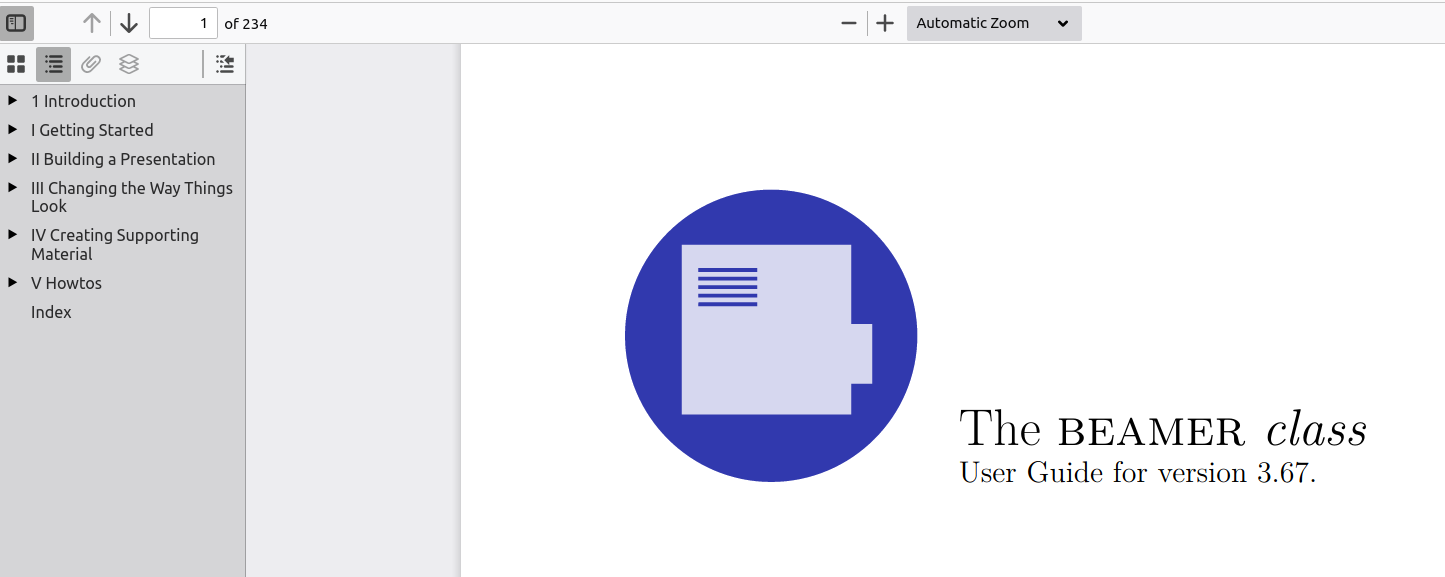
\includegraphics[height=6cm]{beamer-manual}
	\note{This is the manual for the Beamer, the document class for slide decks. It's not the full LaTeX manual, it's just for slides. I want to draw your attention to the upper left hand corner -- that's 234 pages. Of manual. Just for slides!}
\end{frame}

\begin{frame}
	What is \LaTeX{}?
\end{frame}

\begin{frame}
	What is... TeX?
	\note{wikpedia sez: "is a typesetting system which was designed and written by Donald Knuth[1] and first released in 1978. TeX is a popular means of typesetting complex mathematical formulae; it has been noted as one of the most sophisticated digital typographical systems."}
\end{frame}

\begin{frame}
	The \textbf{structure} of a \LaTeX{} document.
	\note{a LaTeX document is *just text*. You can edit it with anything that edits plain text and doesn't mangle it, you can put it in version control, you can copy it anywhere, you can be assured that -- as plain text -- it will probably be viewable, at least as text, for the forseeable future (my lifetime, if not yours at least)}
\end{frame}

\begin{frame}
	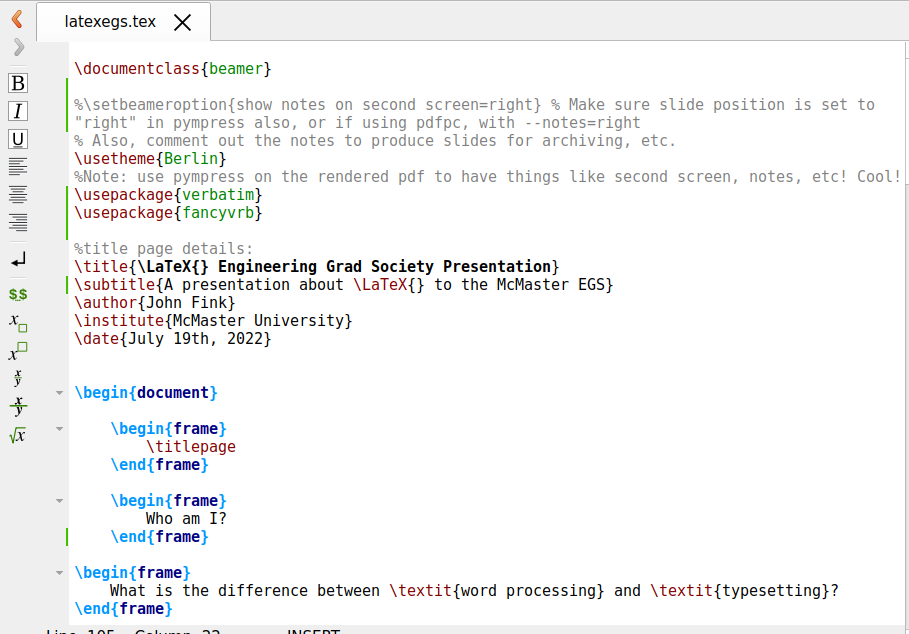
\includegraphics[height=8cm]{latex-structure}
	\note{Let's take a look here. This is the beginning of my slide deck for this very talk -- yup, that's right, you can actually write slides in LaTeX just like any other document. First, you have the preamble -- this sets up your document. Let's go through it, shall we?}
\end{frame}

\begin{frame}[fragile=singleslide]
\begin{Verbatim}
\documentclass{beamer}
\usetheme{Berlin}
\usepackage{verbatim}
\usepackage{fancyvrb}
%comments start with a % sign.
\end{Verbatim}
\note{Beamer includes a lot of packages by default so when you write a paper in LaTeX you might find yourself using way more usepackage statements -- for example, including graphics is not a default package in many LaTeX document classes}.
\end{frame}


\begin{frame}[fragile=singleslide]
	%Verbatim here instead of verbatim as Verbatim is fancyvrb, which I needed for font size changes. Phew!
	\begin{Verbatim}[fontsize=\small]
%title page details:
\title{\LaTeX{} Engineering Grad Society Presentation}
\subtitle{A presentation about \LaTeX{} to the McMaster EGS}
\author{John Fink}
\institute{McMaster University}
\date{July 19th, 2022}
	\end{Verbatim}
	\note{The percent is a comment, of course. Title is title of the presentation -- could be title of a paper or a book, but we're using Beamer, so it's a presentation -- a subtitle, the author, the institute, and the date.}
\end{frame}

\begin{frame}[fragile]
	So just about any \LaTeX{} specific markup will look like:
	\begin{itemize}
		\item A \verb|\| character
		\pause
		\item A \textbf{command}, like \textit{includegraphics}
		\pause
		\item \textbf{options} passed to the command, in \verb|[]|, like \verb|[height=8cm]|
		\pause
		\item The information fed to the command, in \verb|{}|, like \verb|{imagename}|
		\pause
		\item So, the command \verb|\includegraphics[height=8cm]{imagename}| will display the image titled \textit{imagename}, scaled to 8cm height.
	\end{itemize}
	\note{Whoof! A lot to take in. Note that, in LaTeX, at least when you're inserting images, you do not specify an image extension -- e.g., no imagename.png or whatever, just imagename.}
\end{frame}

\begin{frame}
	%this is always the last slide
	Any questions?
\end{frame}
	
\end{document}